\documentclass[greek]{beamer}
%\usepackage{fontspec}
\usepackage{amsmath,amsthm}
\usepackage{unicode-math}
\usepackage{xltxtra}
\usepackage{graphicx}
\usetheme{CambridgeUS}
\usecolortheme{seagull}
\usepackage{hyperref}
\usepackage{ulem}
\usepackage{xgreek}

\usepackage{pgfpages}
\usepackage{tikz}
\usetikzlibrary{mindmap,trees}\usetikzlibrary{shapes.geometric, arrows}

  \tikzstyle{startstop} = [rectangle, rounded corners,
  minimum width=3cm,
  minimum height=1cm,
  text centered,
  draw=black,
  fill=red!30]
  \tikzstyle{decision} = [diamond,
  minimum width=3cm,
  minimum height=1cm,
  text centered,
  draw=black,
  fill=green!30]
  \tikzstyle{arrow} = [thick,->,>=stealth]
  \tikzstyle{process} = [rectangle,
  minimum width=3cm,
  minimum height=1cm,
  text centered,
  text width=3cm,
  draw=black,
  fill=orange!30]
\usepackage{tkz-tab}
%\setbeameroption{show notes on second screen}
%\setbeameroption{show only notes}

\setsansfont{Noto Serif}

\usepackage{multicol}

\usepackage{appendixnumberbeamer}

\usepackage{polynom}

\usepackage{pgffor}

\setbeamercovered{transparent}
\beamertemplatenavigationsymbolsempty

\title{Πολυώνυμα}
\subtitle{Πολυωνυμικές Εξισώσεις}
\author[Λόλας]{Κωνσταντίνος Λόλας}
\date{}

\begin{document}

\begin{frame}
 \titlepage
\end{frame}

\section{Θεωρία}
\begin{frame}{Ότι μάθατε μάθατε, τώρα παιχνίδι!}
 Θα ασχοληθούμε με εξισώσεις!
 \begin{itemize}
  \item<1-> 1ου βαθμού
  \item<2-> 2ου βαθμού
  \item<3-> $ν$ βαθμού με $ν\ge 3$
 \end{itemize}
 \only<4>{χωρίς να μάθουμε τίποτα καινούριο!!!}
\end{frame}

\begin{frame}{Τα άχρηστα που έχουμε μάθει?}
 Κάποτε κάποιος σας είπε ότι η παραγοντοποίηση είναι σημαντική!
 \begin{itemize}
  \item<1-> για 1ου βαθμού? \only<2> {δεν χρειάζεται!}
  \item<2-> για 2ου βαθμού? \only<3> {μόνο όταν μπορούμε!}
  \item<3-> $ν$ βαθμού με $ν\ge 3$? \only<4> {ίσως ο μοναδικός τρόπος}
 \end{itemize}
\end{frame}

\begin{frame}{1ου βαθμού}
 \begin{tikzpicture}
  [level distance=2cm,
   level 1/.style={sibling distance=5cm},
   level 2/.style={sibling distance=5cm},
   edge from parent/.style={->,draw}]

  \node[circle, draw] {$αx+β=0$}
  child {
    node [rectangle,draw] {$x=-\dfrac{β}{α}$, Μοναδική}
    edge from parent
    node[left] {$α\ne 0$}
   }
  child{
    node {$0=β$}
    child {
      node [rectangle,draw] {Ταυτότητα, Άπειρες}
      edge from parent
      node[left] {$β=0$}
     }
    child {
      node [rectangle,draw] {Αδύνατη, Καμία}
      edge from parent
      node[right] {$β\ne 0$}
     }
    edge from parent
    node[right] {$α=0$}
   };
 \end{tikzpicture}
\end{frame}

\begin{frame}{2ου βαθμού}
 \centering
 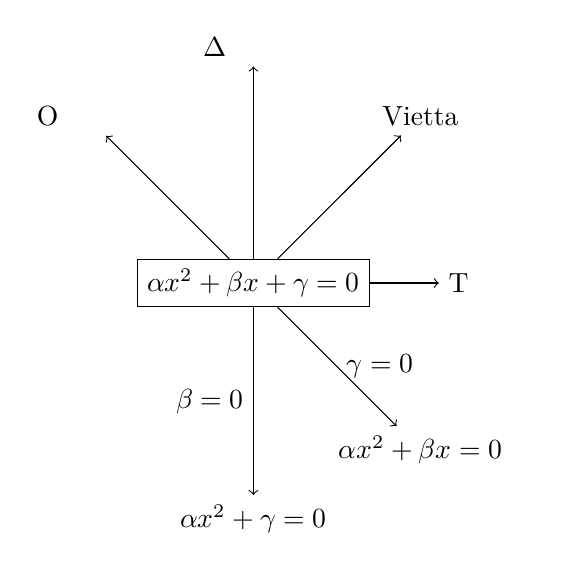
\begin{tikzpicture}
  [level distance=3cm,
   edge from parent/.style={->,draw}]

  \node[rectangle, draw]{$αx^2+βx+γ=0$}
  child[grow=down] {
    node {$αx^2+γ=0$}
    edge from parent
    node[left] {$β= 0$}
   }
  child[grow=south east] {
    node{$αx^2+βx=0$}
    edge from parent
    node[right] {$γ=0$}
   }
  child[grow=east] {
    node{Ταυτότητα}
   }
  child[grow=north east] {
    node{Vietta}
   }
  child[grow=north] {
    node{Διακρίνουσα}
   }
  child[grow=north west] {
    node{Ομαδοποίηση}
   }
  ;
 \end{tikzpicture}
\end{frame}

\begin{frame}{3ου+ ΟΕΟ?}
 Θα ήταν υπέροχο αν μπορούσαμε να το παραγοντοποιήσουμε...
 \begin{itemize}
  \item<1-> Σε 1 πρώτου και 1 δευτέρου?
  \item<2-> Σε 3 πρώτου βαθμού?
 \end{itemize}
\end{frame}

\begin{frame}{4ου ΟΕΟ?}
 Αν μπορούσαμε να το παραγοντοποιήσουμε...
 \begin{itemize}
  \item<1-> Σε 1 πρώτου και 1 τρίτου...?
  \item<2-> Σε 2 πρώτου βαθμού και 1 δευτέρου?
  \item<3-> Σε 2 δευτέρου?
 \end{itemize}
\end{frame}

\begin{frame}{Δηλαδή}
 Μακάρι να πετυχαίναμε ρίζες (και μάλιστα ακέραιες)!
 \begin{block}{Ακέραιες Ρίζες}<2->
  Αν ένα πολυώνυμο με ακέραιους συντελεστές έχει ακέραια ρίζα, τότε η ρίζα αυτή διαιρεί την σταθερά του πολυωνύμου
 \end{block}
 \only<3>
 {$$P(ρ)=0$$ $$α_νρ^ν+α_{ν-1}ρ^{ν-1}+\cdots+α_1ρ+α_0=0$$ $$a_0=-α_νρ^ν-α_{ν-1}ρ^{ν-1}-\cdots-α_1ρ $$ $$a_0=ρ(-α_νρ^{ν-1}-α_{ν-1}ρ^{ν-2}-\cdots-α_1)$$}

\end{frame}

\begin{frame}{Γενικά!}

 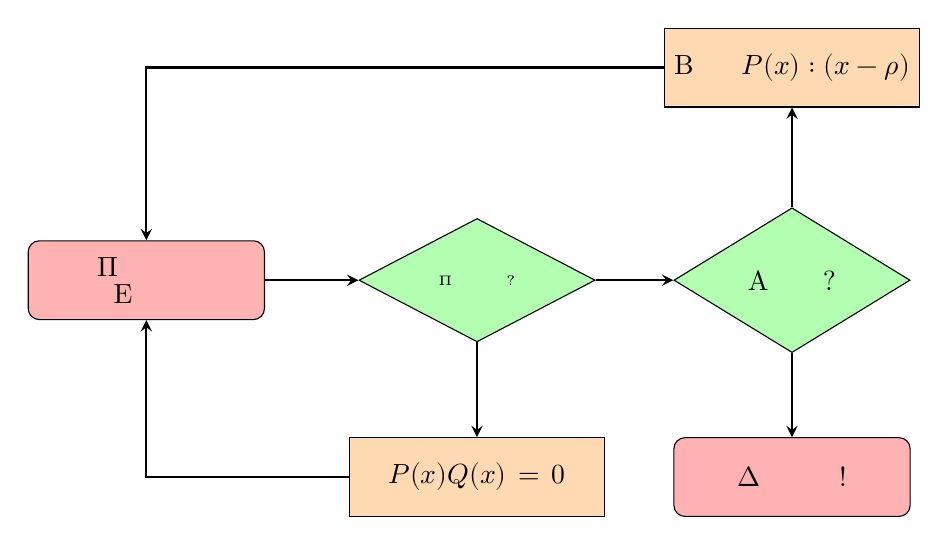
\begin{tikzpicture}[node distance=2cm]
  \node (start) [startstop] {\shortstack{Πολυωνυμική\\ Εξίσωση}};
  \node (dec1) [decision, right of=start, xshift=2.2cm] {\tiny Παραγοντοποίηση?};
  \node (pro1) [process, below of=dec1, yshift=-0.5cm] {$P(x)Q(x)=0$};
  \node (dec2) [decision, right of=dec1, xshift=2cm] {Ακέραιες?};
  \node (pro2) [process, above of=dec2, yshift=0.7cm] {Βρίσκω
   $P(x):(x-ρ)$};
  \node (stop) [startstop, below of=dec2, yshift=-0.5cm] {Δεν λύνεται!};

  \draw [arrow] (start) -- (dec1);
  \draw [arrow] (dec1) -- node[anchor=east] {ναι} (pro1);
  \draw [arrow] (dec1) -- node[anchor=north] {όχι} (dec2);
  \draw [arrow] (pro1) -| (start);
  \draw [arrow] (dec2) -- node[anchor=east] {ναι} (pro2);
  \draw [arrow] (pro2) -| (start);
  \draw [arrow] (dec2) -- node[anchor=east] {όχι} (stop);
 \end{tikzpicture}

 Για κάθε, ΜΑ ΚΑΘΕ πολυώνυμο!
\end{frame}

\section{Ασκήσεις}
\subsection{Άσκηση 1}
\begin{frame}[label=Άσκηση1,t]{Εξάσκηση 1}
 Να λύσετε τις εξισώσεις
 \begin{enumerate}
  \item<1-> $x^4=8x$
  \item<2-> $x^3-2x^2-9x+18=0$
 \end{enumerate}

 % \hyperlink{Λύση1}{\beamerbutton{Λύση}}
\end{frame}

\subsection{Άσκηση 2}
\begin{frame}[label=Άσκηση2,t]{Εξάσκηση 2}
 Να βρείτε τις ακέραιες ρίζες της εξίσωσης $x^3-5x+2=0$

 % \hyperlink{Λύση2}{\beamerbutton{Λύση}}
\end{frame}

\subsection{Άσκηση 3}
\begin{frame}[label=Άσκηση3,t]{Εξάσκηση 3}
 Να δείξετε ότι η εξίσωση $x^3+3x+2=0$ δεν έχει ακέραιες ρίζες.

 % \hyperlink{Λύση3}{\beamerbutton{Λύση}}
\end{frame}

\subsection{Άσκηση 4}
\begin{frame}[label=Άσκηση4,t]{Εξάσκηση 4}
 Να λύσετε την εξίσωση $x^3-3x+2=0$

 % \hyperlink{Λύση4}{\beamerbutton{Λύση}}
\end{frame}

\subsection{Άσκηση 5}
\begin{frame}[label=Άσκηση5,t]{Εξάσκηση 5}
 Να λύσετε την εξίσωση $2x^4-3x^3-17x^2+27x-9=0$

 % \hyperlink{Λύση5}{\beamerbutton{Λύση}}
\end{frame}

\subsection{Άσκηση 6}
\begin{frame}[label=Άσκηση6,t]{Εξάσκηση 6}
 Να λύσετε την εξίσωση $x^6-7x^2-6=0$

 % \hyperlink{Λύση6}{\beamerbutton{Λύση}}
\end{frame}

\subsection{Άσκηση 7}
\begin{frame}[label=Άσκηση7,t]{Εξάσκηση 7}
 Να βρείτε τα κοινά σημεία της γραφικής παράστασης της συνάρτησης $f(x)=-x^3-x+2$ με τον άξονα $x'x$

 %\hyperlink{Λύση7}{\beamerbutton{Λύση}}
\end{frame}

\subsection{Άσκηση 8}
\begin{frame}[label=Άσκηση8,t]{Εξάσκηση 8}
 Να βρείτε τα κοινά σημεία των γραφικών παραστάσεων των συναρτήσεων $$f(x)=x^3+9$$ και $$g(x)=5x^2-3x$$

 %\hyperlink{Λύση8}{\beamerbutton{Λύση}}
\end{frame}

\subsection{Άσκηση 9}
\begin{frame}[label=Άσκηση9,t]{Εξάσκηση 9}
 Αν η εξίσωση $x^3-(λ+2)x^2+2λx-1=0$, $λ\in\mathbb{Z}$ έχει ακέραια ρίζα, να βρείτε το $λ$ και μετά να λύσετε την εξίσωση.

 %\hyperlink{Λύση9}{\beamerbutton{Λύση}}
\end{frame}

\subsection{Άσκηση 10}
\begin{frame}[label=Άσκηση10,t]{Εξάσκηση 10}
Να λύσετε την εξίσωση $(3x+1)^8-15(3x+1)^4-16=0$

 %\hyperlink{Λύση10}{\beamerbutton{Λύση}}
\end{frame}

\subsection{Άσκηση 11}
\begin{frame}[label=Άσκηση11,t]{Εξάσκηση 11}
 Να λύσετε την εξίσωση $(x^2-x-1)^2-6(x^2-x-3)-7=0$

 %\hyperlink{Λύση11}{\beamerbutton{Λύση}}
\end{frame}

\subsection{Άσκηση 12}
\begin{frame}[label=Άσκηση12,t]{Εξάσκηση 12}
 Να λύσετε την εξίσωση $6x^4+5x^3-38x^2+5x+6=0$

 %\hyperlink{Λύση12}{\beamerbutton{Λύση}}
\end{frame}


% \appendix
%
% \section{Αποδείξεις}
% \begin{frame}[label=Απόδειξη1]{Απόδειξη μονοτονίας συνάρτησης}
%  Θα δείξουμε ότι για κάθε $x_1<x_2\in Δ \implies f(x_1)<f(x_2)$.
%
%  \onslide<1-> Στο $[x_1,x_2]$ είναι παραγωγίσιμη, άρα θα ισχύει το ΘΜΤ
%
%  \onslide<2-> Υπάρχει $ξ\in Δ$ ώστε $f'(ξ)=\dfrac{f(x_2)-f(x_1)}{x_2-x_1}$.
%
%  \onslide<3-> Αλλά $f'(x)>0$ για κάθε $x\in Δ$
%
%  \onslide<4-> Άρα $f'(ξ)=\dfrac{f(x_2)-f(x_1)}{x_2-x_1}>0$
%
%  \onslide<5-> $f(x_2)>f(x_1)$
%
%  \hyperlink{Θεώρημα1}{\beamerbutton{Πίσω στη θεωρία}}
% \end{frame}


% \section{Λύσεις Ασκήσεων}
% \begin{frame}
%  \tableofcontents
% \end{frame}
%
% \subsection{Άσκηση 1}
% \begin{frame}[label=Λύση1]
%  Με θεώρημα ενδιαμέσων τιμών. Η συνάρτηση είναι συνεχής στο $[10,11]$ με $f(10)=1024$ και $f(11)=2048$. Αφού $2023\in (1024,2048)$ υπάρχει $x_0$...
%
%  \hyperlink{Άσκηση1}{\beamerbutton{Πίσω στην άσκηση}}
% \end{frame}
%
% \subsection{Άσκηση 2}
% \begin{frame}[label=Λύση2]
%  Με Bolzano ή με μέγιστης ελάχιστης τιμής και ΘΕΤ.
%
%  \begin{gather*}
%   f(3)<f(2)<f(1) \\
%   3f(3)<f(1)+f(2)+f(3)<3f(1) \\
%   f(3)<\dfrac{f(1)+f(2)+f(3)}{3}<f(1)
%  \end{gather*}
%
%  \hyperlink{Άσκηση2}{\beamerbutton{Πίσω στην άσκηση}}
% \end{frame}
%
% \subsection{Άσκηση 3}
% \begin{frame}[label=Λύση3]
%  Προφανές ελάχιστο στα $x_1=1$ και $x_2=3$. Ως συνεχής στο $[1,3]$ έχει σίγουρα ΚΑΙ μέγιστο στο $(1,3)$
%
%  \hyperlink{Άσκηση3}{\beamerbutton{Πίσω στην άσκηση}}
% \end{frame}
%
% \subsection{Άσκηση 4}
% \begin{frame}[label=Λύση4]
%  Η συνάρτηση `απόστασης` $f(x)-x$ είναι ορισμένη στο κλειστό διάστημα και έχει σίγουρα μέγιστο
%
%  \hyperlink{Άσκηση4}{\beamerbutton{Πίσω στην άσκηση}}
% \end{frame}
%
% \subsection{Άσκηση 5}
% \begin{frame}[label=Λύση5]
%  Όμοια με την Άσκηση 2
%
%  \hyperlink{Άσκηση5}{\beamerbutton{Πίσω στην άσκηση}}
% \end{frame}
%
% \subsection{Άσκηση 6}
% \begin{frame}[label=Λύση6]
%  \begin{enumerate}
%   \item Είναι γνησίως αύξουσα άρα $(f(+\infty),f(-\infty))$
%   \item Προφανώς $[f(0),f(1)]$...
%  \end{enumerate}
%
%  \hyperlink{Άσκηση6}{\beamerbutton{Πίσω στην άσκηση}}
% \end{frame}

\end{document}
